\documentclass[a4paper,twocolumn]{jsarticle}
%\documentclass[a4j,twocolumn]{jarticle} % 'jsarticle' が使えない場合はこちらを利用

% 上記 documentclass のオプションは自由に追加してもよい。

%%%%%%%%%%%%%%%%%%%%%%%%%%%%%%%%%%%%%%%%%%%%%%%%%%%%%%%%%%%%%%%%%%%%%%%%%%%%%%
%%% ページ設定 (この項目は論文著者は編集しないこと。)

% 芸術科学会学術会議用スタイルパッケージ
\usepackage{artsci-conf-j} 

%%%%%%%%%%%%%%%%%%%%%%%%%%%%%%%%%%%%%%%%%%%%%%%%%%%%%%%%%%%%%%%%%%%%%%%%%%%%%%
%%% パッケージ一覧 (必要なパッケージを任意に追加してよい)

\usepackage{amsmath, amssymb}	% AMS-LaTeX
\usepackage[dvipdfmx]{graphicx}	% 「graphics」パッケージに変更してもよい。
\usepackage{float}		% 図表が記述位置から飛ばないためのパッケージ
\usepackage{url}

%%%%%%%%%%%%%%%%%%%%%%%%%%%%%%%%%%%%%%%%%%%%%%%%%%%%%%%%%%%%%%%%%%%%%%%%%%%%%%
%%% マクロ一覧 (必要なマクロをこの部分に記述)

\newcommand{\bA}{\mathbf{A}}
\newcommand{\bB}{\mathbf{B}}



%%%%%%%%%%%%%%%%%%%%%%%%%%%%%%%%%%%%%%%%%%%%%%%%%%%%%%%%%%%%%%%%%%%%%%%%%%%%%%
%%% 図ファイルのパス設定

\graphicspath{{fig/}}

%% タイトル,概要,キーワードなど
%%%%%%%%%%%%%%%%%%%%%%%%%%%%%%%%%%%%%%%%%%%%%%%%%%%%%%%%%%%%%%%%%%%%%%%%%%%%%%
%%% タイトル、著者、所属、概要

% 日本語タイトル
\jtitle{
レトロネーザルアロマを利用した \\
味覚の拡張(\LaTeX 版)
}

% 英語タイトル
\etitle{
Expressive Japan \\
Sample Style (\LaTeX Version)
}

% 日本語著者
% 共著者氏名の間隔は ~ や \quad 等で適宜調節のこと。
\jauthor{
濱家陸\({}^\dagger\) \quad
}

% 英語著者
\eauthor{
Riku Hamaie\({}^\dagger\) \quad
}

% 日本語所属
\jaffiliation{
\(\dagger\) 東京工科大学 ~~~
	〒192-0982 東京都八王子市片倉町1404-1 \\
\(\ddagger\) 東京工科大学メディア学部 ~~~
	〒192-0982 東京都八王子市片倉町1404-1
}

% 英語所属
\eaffiliation{
\(\dagger\) Graduate School of Bionics, Computer and Media Sciences,
	Tokyo University of Technology \\
\(\ddagger\) School of Media Science,
	Tokyo University of Technology
}

% 連絡先電子メールアドレス
% (
% このサンプルでは「@」を2バイト文字にすることで対応してある。)
\email{
m01172238c@edu.teu.ac.jp
}

% 日本語概要
\jabstract{
嗅覚は味の知覚に密接に関わり影響を与えている.
風味に着目し,密接に関わっている口内から入る香り(レトロネーザル)を利用した.
レトロネーザルで感じた風味は味を感じ方に大きな影響を与えると考え,舌で感じる味覚ではなく嗅覚から感じる風味に焦点をあてた実験を検証した。
口の中からの嗅覚刺激を用いて香りを提示することで, 風味を与えることができるのではないかと考え,香りを閉じこめた直径 3 センチメートルのゼリーを食べることで,風味を想起させることが出来るかを検討した.
被験者に風味を感じることができるかを判断してもらい,風味提示ゼリーの有用性を示した.	
}

% 英語概要
\eabstract{
This article is to provide LaTeX sample for posting of ``Expressive Japan''.
This sample is created with emphasis on consistency with the sample of
the journal of the Society of Art and Science.
}

% 日本語キーワード
\jkeyword{
嗅覚, 味覚, 香り, 風味
}

% 英語キーワード
\ekeyword{
LaTeX, article, template, society
}


%%%%%%%%%%%%%%%%%%%%%%%%%%%%%%%%%%%%%%%%%%%%%%%%%%%%%%%%%%%%%%%%%%%%%%%%%%%%%%
% ここより論文本体
\pagestyle{empty}

\begin{document}
\maketitle

\section{はじめに}
\subsection{人間の嗅覚}
\label{subsec:intro}
人間の食べる時に使う感覚は舌による味覚だけではなく,嗅覚,視覚,聴覚,触覚の五感すべて
によって刺激から感じる. 本研究では,その中でも味覚に注目して,味覚に関係性が深い嗅覚に
着目した.嗅覚は,食べ物の香りを感じる時にとても敏感に働く感覚である.食べる前に香りを
嗅ぐと,食欲を増大させる.他に,食事の良し悪しや好き嫌いを判断する時にも,必要となる感
覚である.そのため,物を食べるときは,味覚で感じている前に食に対しての情報を感じとる感
覚である.その情報が味覚の感覚に影響を与え,感じ方を変化させるため「味」に大きな影響を
与えていると言われている.嗅覚には 2 つの嗅覚経路を通ることで嗅状皮細胞にたどり着く.一
つ目は鼻から入る経路で,一般的に匂いを嗅ぐときに使う嗅感覚である.二つ目は口から入り鼻
から抜けて出ていく経路で,食べ物を食べた時や口の中に入れた時に生じるものである.嗅覚は
嗅状皮細胞が特定の化学物質に触れ合うことで香りを認識する.この二つの嗅覚から味や匂いの
感覚を認識している.


\subsection{オルソネーザルアロマとレトロネーザルアロマ}
嗅覚には図\ref{kyukaku}で示したようにオルソネーザルと言われる鼻から入る香りとレトロネーザルと
言われる口から入り鼻から抜ける香りの2つがある.鼻をつまむと味がしなくなる現象や風邪な
ど鼻の不具合により味がしなくなる現象から嗅覚は味覚に影響があることが分かる.オルソネー
ザルの場合は,鼻から生じる単独の感覚であり,香りに特化した知覚である.一方,レトロネー
ザルは口内から入るため,味覚や感覚,触覚も加わることから複数の感覚が連動して新たな風味
が形成される.


\begin{figure}[t]
    \centering
    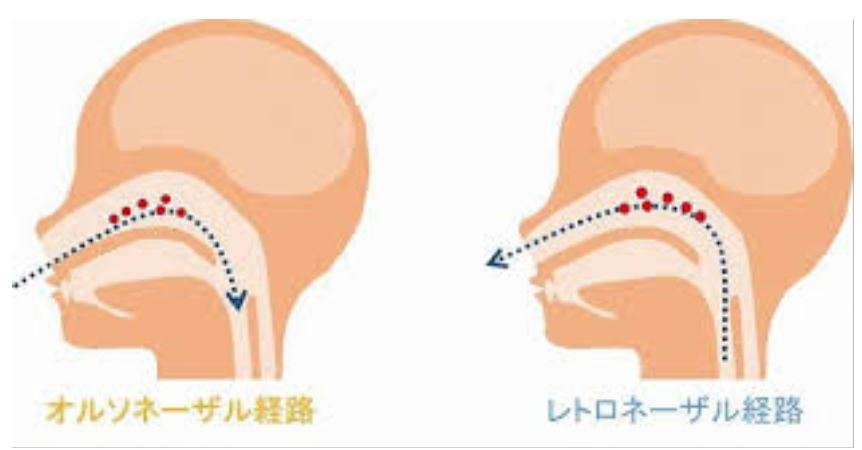
\includegraphics[width = 0.7\columnwidth]{kyukaku.JPG}
    \caption{オルソネーザルとレトロネーザル}
    \label{kyukaku}
  \end{figure}


\subsection{研究の目的}
レトロネーザルはオルソネーザルよりも複数の感覚から風味を感じやすいと考える.そのため
レトロネーザルを利用し,口の中から香りを与え嗅覚に刺激を与えることで風味を感じさせるこ
とが出来ると考えた.このように嗅覚刺激による風味,味覚への変化を検証する研究は存在する
が,食べられるものを使い香りを与えるものは少ない.チューブによって香りを嗅覚に与えるデ
バイスが多いため,食べれるものでの仕組みを作り出すことで口の中にチューブを入れるなどの
問題点を解決できるのではないかと考えた.


本稿では,口の中に香りを与える方法として,アガーで作成したゼリーの中に香りを閉
じこめたものを用意した.無味無臭の球体のゼリーの中に香りを閉じこめることで,口の中に香
りを与えることができると考えた.この香りによって人間が飲食するときにおいて感じる風味を
与えることができる.この仕組みにより風味にどのような差異があるか調査し,研究をしていく.
\section{関連研究}

実際にそれらの関係性を
利用した研究は行われている.
角谷らの呼吸と連動した醤油の匂い提示による塩味増強
効果\cite{enmi}ではレトロネーザルに着目しており,刺激提示装置は
呼吸センサを伴う前後鼻腔経路嗅覚デバイスを用いた. 
前鼻腔経路に刺激を提示するときは吸気,
後腔経路に提示するときは呼気に合わせて刺激を
提示することにより,食べ物の風味を増強させることが出
来ることを示した.


また,岡崎らの嗅覚ディスプレイ\cite{hasi}は,レトロネーザルに
に着目し,箸の先から香りをだし口内に入れることで,風味
を増強させることが出来ると示した.


一方で鳴海らによるメタクッキー\cite{narumi2}は味覚に対して,オル
ソネーザルと視覚による刺激を用いる. プレーン味のクッ
キーに対して HMD を用いた見た目の違うクッキーに見せ,
オルソネーザルの嗅覚刺激で別の味のクッキーの香りをエ
アポンプによる空気の送風で香りかがせる. 視覚と嗅覚を
用いることでの味の変化がある回答を得ている.


白須らはオルソネーザルからの嗅覚刺激を利用した風味
変容の研究\cite{fan}\cite{pomp}を行っており,「かき氷」を題材とし,味覚変容
の手法を検討している. かき氷のシロップを容器に LED
光源を取り付けることでシロップの色を再現し,スプーン
から香料を出すことで鼻に直接香りを与える. 視覚的に着
色料ではなく光源をを使用することで,リアルタイムで同
じ皿で視覚情報と嗅覚情報を切り替えるシステムを作成し
ている. 視覚と鼻からの嗅覚刺激を用いることでの味覚の
変化の有用性を示した。

\section{予備実験}
口から鼻に抜ける香り(オルソネーザル)からの嗅覚情報の提示方法として,アガーを使用し
たゼリーを用いた.アガーを使用したゼリーを球体に固め,その中身を空洞にすることで空気を
入れるスペースが出来る.スペースに香りを閉じこめることで香りを閉じこめたゼリーを作成し
た.そのゼリーを口から食べることで口の中でゼリーが割れることにより,閉じこめられていた
香りが出て鼻から抜ける香りを与える物となっている.

\subsection{球体ゼリーの作成方法}
中に香りを閉じこめるためには,ゼリーの中身を空洞にする必要がある.そのため,ゼリーを
作成するための材料といてアガーを使用した.今回アガーを利用した理由は,ゼラチンよりも透
明度が高く,常温でも溶けない性質を持っているからである.また,アガー自体には味がついてお
らずゼリー状に固めても無味無臭で作ることが出来る.もう一つの特徴として,溶ける温度が 90
℃以上と溶けにくく,固まる温度が 30,40 ℃と常温でも固まりすぐに固めることが出来るため
扱いやすく丈夫である.固める際に図 4.1 で示した丸い氷を作成する用の製氷機を使用した.こ
の製氷機にアガーを溶かしたゼリーの素となる液体を半分まで流し込む.アガーの固まる温度は
30,40 度のため,製氷機を回しながら氷で全体を急速に冷やすことで型にそって固まり,図 4.3
19
で示したような中が空洞で球体のゼリーを作成している.


\subsection{香りの注入方法}
 香りを注入する方法としては注射器の中に香料を含めたコットンを入れ,注射器内に香りを
含めることで構成した.空洞があるゼリーに香りを閉じこめるために,大きな穴が開かないよう
に図 4.2 で示した細い針の注射器を使用した.元々空洞に空気がはいっているため注射器でゼ
リーの空洞の空気を抜くことにより中に香りをこめた空気が入るようにして,注射器で香りを空
洞の中に注入した.香りは注射器の中に香料を含めたコットンを入れ,注射器内に香りを含める
ことで構成することで香りを閉じこめた.


\subsection{嗅覚提示実験方法}
 予備実験では香りを閉じこめたゼリーを食べることで,風味を想起させることが出来るかを
検証する.香りを想起させるために香りの感じ方が強い二つの香りを用意した.甘味の強い香り
と塩味が強い香りの香料を使用する.今回の実験では,作成した嗅覚提示ゼリーの有用性を調査
するとともに,中に入れる香りがどの程度の認知を得るか調査した.

\subsection{香料}
香料は甘味の強い香りのバニラと塩味が強い香りの醤油の香料を用意する.香料はコットンに
染み込ませ注射器の中に入れることで気化し香りが充満し,濃度が高い香りを注入することがで
きると考えた.また,今回はゼリーを口の中に入れた際に香りを感じることが出来るかを調査す
るためゼリー自体の味を無味とする.2 名の風邪などひいておらず,鼻詰まりなど匂いを嗅ぐのに
支障がない被験者に実際に香りを注入したゼリーを食べてもらい,風味を感じるか実験を行った.

\subsection{予備実験結果}
被験者 2 名に行った実験の結果,香りを閉じこめたゼリーを食して,バニラの香り,醤油の香
り 2 種類とも風味を僅かに感じたという結果になった.香料の違いでの感覚の差ではなく,香料
の量と濃度がある程度必要なことを示した.また,意見として「無味のゼリーの味が邪魔してい
た」ということから,ゼリーの味付けが無味だと不快感が出てしまうことが明らかになった.
上記の結果から,今回作成したゼリーを用いた嗅覚提示は僅かながら,風味を与える可能性を
感じさせるものである.だが,香りの量,濃度が不十分なため風味が僅かになってしまったため,
香料での香りの出し方と量を増強させる必要があると考える.そのため,コットンに香りをつけ
る量やゼリーの大きさを調整しながら,香りの質を高めることにより感じ方が強化できるのでは
ないかと考えた.また,ゼリー自体の味付けに関して無味だと不快感を感じることから,中に閉
じこめた香りの嗅覚刺激だけでなく,ゼリー自体に甘味や塩味をつけ味覚刺激を与え調査する必
要があると考える.

\section{実験}

口から鼻に抜ける香り(レトロネーザル)からの嗅覚情報の提示方法として,アガーを使用し
たゼリーを用いた.アガーを使用したゼリーを球体に固め,その中身を空洞にすることで空気を
入れるスペースが出来る.スペースに香りを閉じこめることで香りを閉じこめたゼリーを作成し
た.そのゼリーを口から食べることで口の中でゼリーが割れることにより,閉じこめられていた
香りが出て鼻から抜ける香りを与える物となっている.

\subsection{風味変容システムの概要}

嗅覚情報を風味として付与する仕組みとして,
香りの付いた液体を熱する事で出る蒸気を吸い,
その香りを楽しむVapeの香料の液体であるリキッドを
使用した.
気化させた香料を中に閉じこめる風味強化した新たなシステムを試作している.アルコー
ルのような気化しやすい液体を混ぜて中に入れゼリーの中で気化して充満させることでより香料
の濃度を上がることが出来ると考えた.


\subsection{ゼリーの大きさと作成}

中に香りを閉じこめるためには,ゼリーの中身を空洞にする必要がある.そのため,ゼリーを
作成するための材料といてアガーを使用した.今回アガーを利用した理由は,ゼラチンよりも透
明度が高く,常温でも溶けない性質を持っているからである.また,アガー自体には味がついてお
らずゼリー状に固めても無味無臭で作ることが出来る.もう一つの特徴として,溶ける温度が 90
℃以上と溶けにくく,固まる温度が30,40℃と常温でも固まりすぐに固めることが出来るため
扱いやすく丈夫である.固める際にで示した丸い氷を作成する用の製氷機を使用した.


ゼリーは直径3センチメートルの大きさの製氷機を使用し作成した.
安全に口内に入れやすく香料を入れる容量があるで示した直径3センチメー
トルの製氷機を使用した.


また,ゼリーを作成するにおいて予備実験から強度が弱く中に香りを入れる際に穴を開けるた
め潰れてしまう問題点が存在した.そのため,強度が強いものにするために氷水で5分間冷や
した後冷蔵庫で冷やすことでより図\ref{zeri}で示した強度の強いゼリーを作り出すことができた.ゼ
リー作成方法は以下のようになっている.


1.  アガー 5g を鍋に入れ,水 100ml を少しずつ混ぜながら加える.


2.  完全に解けたら火にかける.沸騰したら火を止める.


3. 2 の液体を立体の体積の半分よりやや少なめに入れる.


4.  フタをして,開かないように固定.


5.  容器を氷水の中で5分ほど回す. この時に一定方向だけでなく縦横斜めと全体にいきたわるように回す.


6.  冷蔵庫で冷やしておく. 冷やしておく事でゼリーがより固まり取り出しやすくなる.



  \begin{figure}[t]
    \centering
    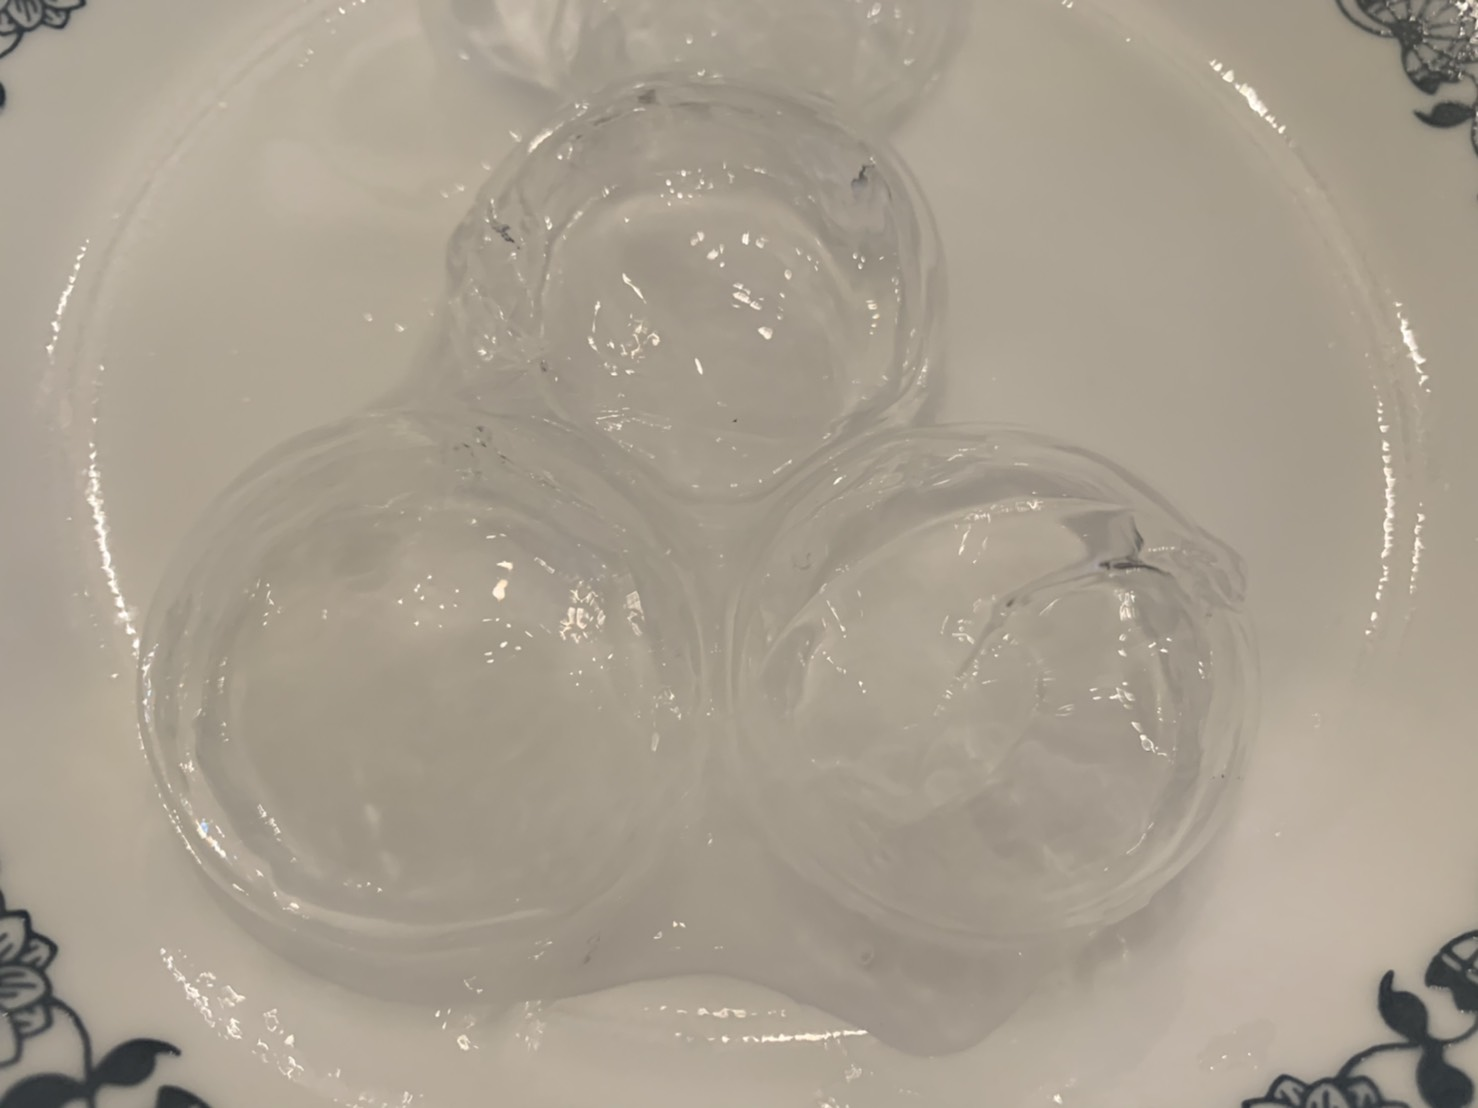
\includegraphics[width = 0.7\columnwidth]{zeri2.jpg}
    \caption{空洞のあるゼリー}
    \label{zeri}
  \end{figure}


\subsection{香りの注入方法}
  空洞があるゼリーに香りを閉じこめるために,大きな穴が開かないよう
に図\ref{tyusya}で示した細い針の注射器を使用した.元々空洞に空気がはいっているため注射器でゼ
リーの空洞の空気を抜くことにより中に香りをこめた空気が入るようにして,注射器で香りを空
洞の中に注入した.

\begin{figure}[t]
  \centering
  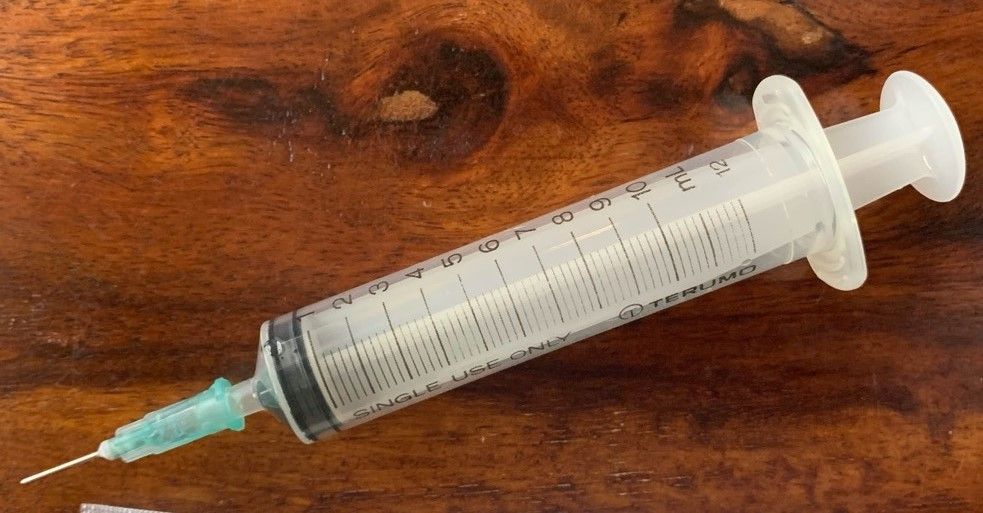
\includegraphics[width = 0.8\columnwidth]{tyusya1.jpg}
  \caption{香りを注入する注射器}
  \label{tyusya}
\end{figure}


\subsection{実験の方法}

本実験では香りを閉じこめた直径3センチメートルのゼリーを食べることで,風味を想起させ
ることが出来るかを検討する.香りを想起させるためにVapeの香りがわかりやすいリキッド二
つの香りを用意した.なお,口内で香りを充満させ風味を感じさせるために食べる際にゼリーを
口内で割るよう一口で口内に入れてもらう.この時に舌に当たる味ではなく鼻から向ける風味を
感じることができるかを判断してもらう.今回の実験では,作成した嗅覚提示ゼリーの有用性を
調査するとともに,中に入れる香りがどの程度の認知を得るか調査した.


今回実験するにあたって四種類のゼリーを用意した.香料を気化させた空気を注射器で吸い取
り,空洞のゼリーに入れたものを青りんごの Vape リキッドとバニラエッセンスの二
種類用意した.この青りんごの香りを含んだゼリーを1のゼリー,バニラの香りを含んだゼリー
を2のゼリーとする.


また,香料をゼリーの中に入れ,ゼリー内で気化させ中に香りを充満させる方法で青りんごの
Vapeリキッドとバニラエッセンスの二種類用意した. この青りんごの香りを含んだゼリーを3の
ゼリーバニラの香りを含んだゼリーを4のゼリーとする.
この四種類の香りの入ったゼリーを食してもらい風味の感じ方を調査した.
\section{結果と考察}

\subsection{評価方法}

風味を感じさせる四つの種類の中に香りが入っているゼリーを食べてもらい風味の感じ方を検
証する.システムにより一瞬でも風味を想起しか確認するために
4段階評価(1:全く感じない~4:すごく感じる)で変化の
度合いを調査する.さらに,自由記述でコメントを記入してもらうこととした.アンケートの回
答は風邪などひいておらず,嗅覚,味覚が正常な状態である6名の被験者を用意した.

実験結果を図\ref{gurafu}示す.


\begin{figure}[t]
    \centering
    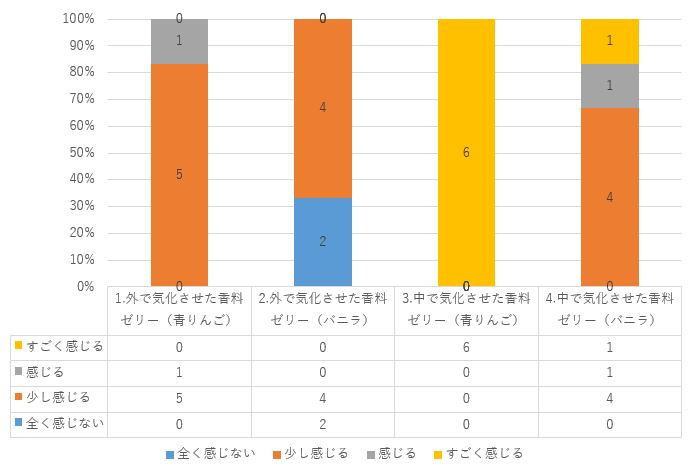
\includegraphics[width = 1.0\columnwidth]{gurafu1.JPG}
    \caption{風味の感じ方アンケート結果}
    \label{gurafu}
  \end{figure}


\subsection{実験結果と考察}

気化した香りを入れた場合の香りは,青りんごのVapeのリキッドとバニラエッセンス二つと
も少し感じたが多数であった.これは,気化した香りを入れた仕組みでは香りの量が少なく風味
を感じることが難しいという結果になった.


また,青りんごのVapeリキッドにおける評価は全員がすごく風味を感じたという結果であっ
た.バニラエッセンスは少し感じたという人が多数であった.これは香りが強いVapeのリキッ
ドは口内から鼻に抜ける風味を感じやすいと思われる.一方バニラエッセンスは香りが分かりに
くいため少し感じづらい結果になったと考える.これは,リキッドをゼリーの中で気化させる仕
組みが有効であったと言える.このことから,風味の感じ方に関しては気化した香りを入れるよりも,
ゼリーの中で気化させ香りを充満させる方が優位性が高いのではないかと考えられる.


自由記述では,「青りんごの香りが口の中から鼻に抜けるのを感じた」「味がないとおいしくは
ない」「ガムのような味」と言った様々な意見が得られた.


これらの結果から,レトロネーザルの嗅覚における影響に対しての仮説が生まれた.それは,
一つ目に青りんごのような風味を想像しやすい香りの方が風味を感じやすいのではないかという
考察が生まれた.バニラは普段口にする際,香りだけではなく甘い味がついていることがほとん
どのため香りだけで判断することが難しいと考えられる.


二つ目に,気化する量がカギになっているのではないかという仮説が生まれた.今回予備実験
で風味をあまり感じることが難しかったため,気化しやすく,香りが強いVapeのリキッドを使用
した.そのため,ゼリー内で気化した香りの量が増え,風味を感じやすくなったと考えられる.
\section{おわりに}

本研究では,レトロネーザルアロマと嗅覚デバイスを利用して,風味の変化を起こすシステム
の検討を行った.そのためにゼリーを用いた風味変容システムを構築した.
このシステムを用いて,ゼリーに対して香りを付与し,食した時の風味を評価してもらう実験
を行った.その結果,風味の変化を感じているという結果が得られ,口内に入れたときの風味を
認識させることができるという有効性を示した.
この手法は,決まった風味だけでなく様々な風味に対して一瞬の風味を想起させることができ
るのではないかと考えている.具体的には,紅茶の風味やフルーツの風味のような香りが想像す
ることができるものでなら行えるのではないかと考えており,今後の検討にしていきたい.
現段階において,香りを入れる際に,そのたびに注射器で香料を入れ替えなければならない.
また,その提示する香りが混ざらないように香料をいれる注射器の容器を分ける事の重要性を改
めて再確認した.今回の実験では香りが混ざらないように香料が付着したものは香料ごとに分け
保管し,洗浄していた.加えて,一度香りが部屋に充満してしまうと被験者が余計な香りに気づ
き誤差を生じてしまう可能性があった.異なる香りが混ざり合わないよう配慮が必要である.
今後の展望として,今回実験で使用した以外の香料での風味の感じ方を検証していきたいと考
えている.香料にはフルーツだけではなく,
様々な香料での風味の感じ方の比較実験を実践していくことが必要である.
また,味覚や視覚を組み合わせたときに風味の感じ方と味覚への影響の変化があるのではないか
と考えている.そして,換気や部品の保管方法の重要性を再確認したところで,実験が行いやす
くするための実験方法を検討している.
以上で述べたことを実践していくことで,レトロネーザルからの風味を認識させることができ
るのではないかと考えている.また,実際に食べなくても嗅覚だけで味を想起することが出来る
体験を感じさせることができる.


\bibliography{bib} % BibTeX ファイル (.bib) を記述
\bibliographystyle{junsrt} % 番号を掲載順にソートする。

\end{document}
